%%%%%%%%%%%%%%%%%%%%%%%%%%%%%%%%%%%%%%%%%%%%%%%%%%%%%%%%%%%%%%%%%%%%%%%%%%%%%%%%%%%%%%%%%%%%%%%%%%%
% Chapter 1 -> Introduction
% Author: Mingbo Cheng
%%%%%%%%%%%%%%%%%%%%%%%%%%%%%%%%%%%%%%%%%%%%%%%%%%%%%%%%%%%%%%%%%%%%%%%%%%%%%%%%%%%%%%%%%%%%%%%%%%%
\chapter{Introduction}
\label{chapter:introduction}

\graphicspath{{chapter1/figs/}}


\section{Motivation}
\label{introduction:sec1.motivation}

Simultaneously studying multimodalities at a single cell like joint profiling chromatin accessibility and gene expression at a single-cell level offers the potential to unravel networks of gene regulation powered by enhancers. Biological processes and systems exhibit dynamism. To comprehensively grasp the molecular and cellular constituents, along with the networks they form during these processes, researchers frequently gather data across temporal intervals. However, there are many obstacles in the process of analyzing single cell multi-modal data. The first challenge is the integration of these modalities is challenging due to the different sparsity of the data and the different characteristics of these modalities. Existing methods for the integration of single-cell multi-omics data are mostly based on matrix factorization, which is not suitable for the integration of sparse data. In addition, these methods do not consider the different characteristics of the two modalities, which may lead to the loss of information. Therefore, there is a need for a new method to integrate single-cell multi-omics data.

\begin{figure}[!ht]
	\centering
	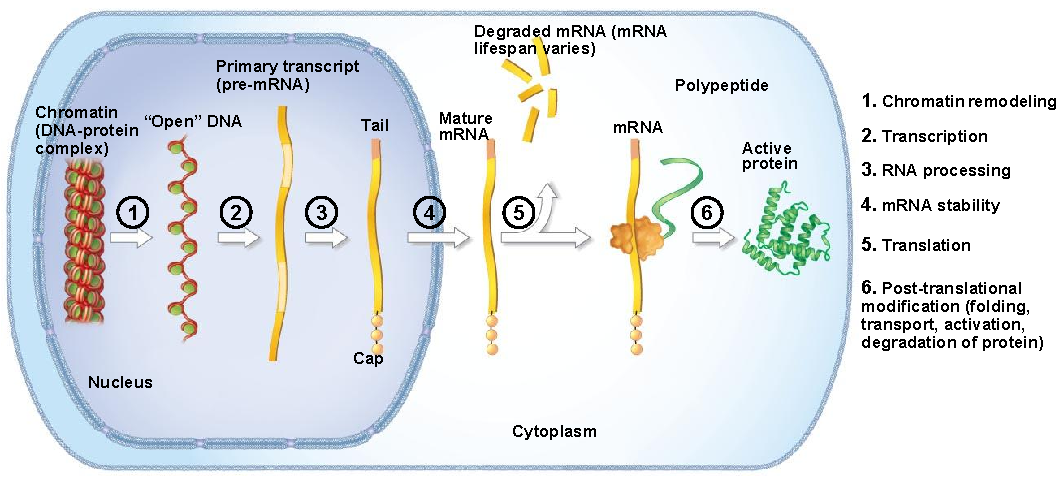
\includegraphics[width=0.95\textwidth]{gene_expression_process/fig}
	\vspace{0.1cm}
	\caption[gene regulation]{gene regulation}
	\label{fig:gene_expression_process}
\end{figure}

\section{Thesis Overview}
\label{introduction:sec2.overview}

\begin{figure}[!ht]
	\centering
	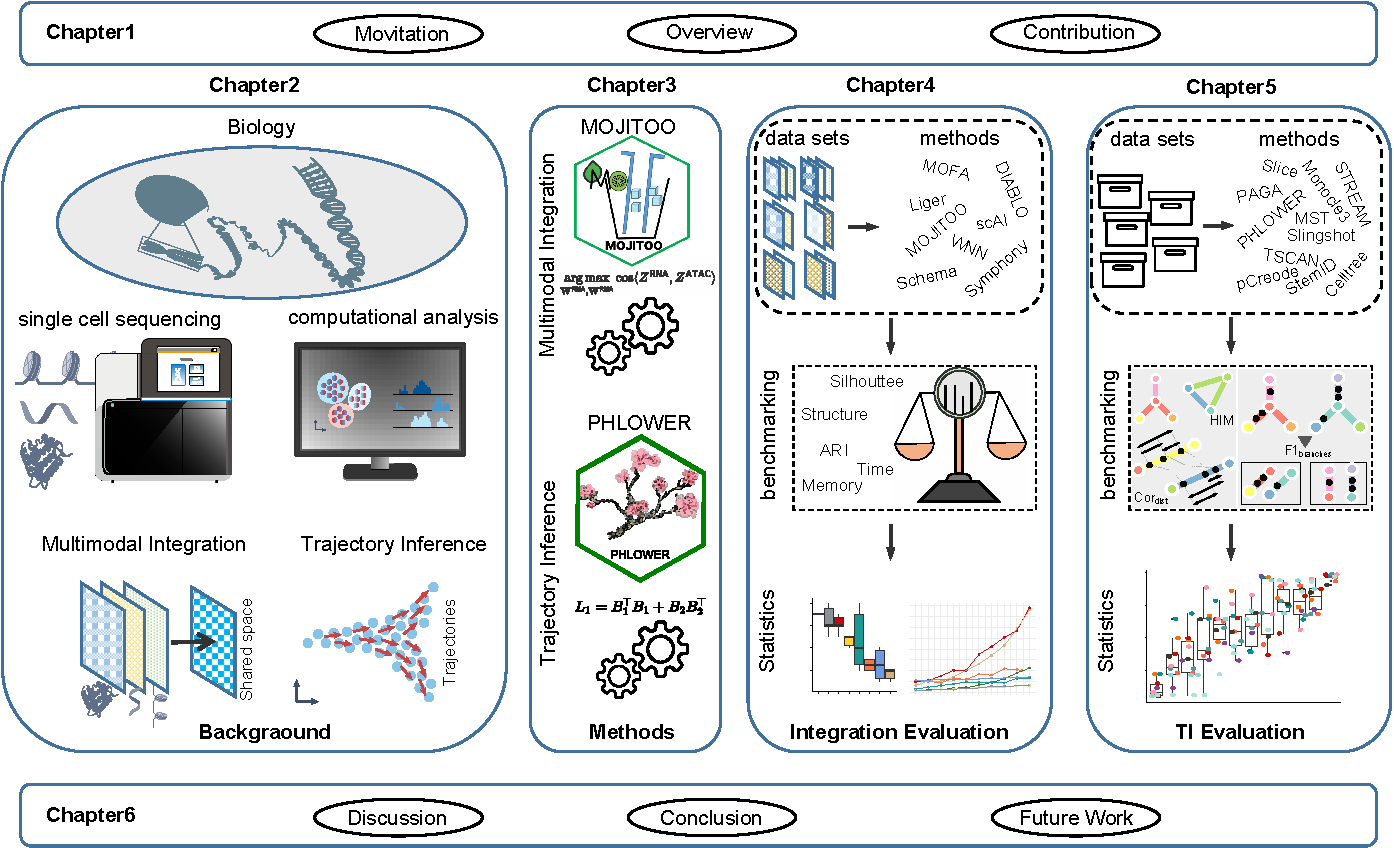
\includegraphics[width=0.95\textwidth]{thesis_overview/fig}
	\vspace{0.1cm}
	\caption[thesis overview]{thesis overview}
	\label{fig:thesis_overview}
\end{figure}

\begin{figure}[!ht]
	\centering
	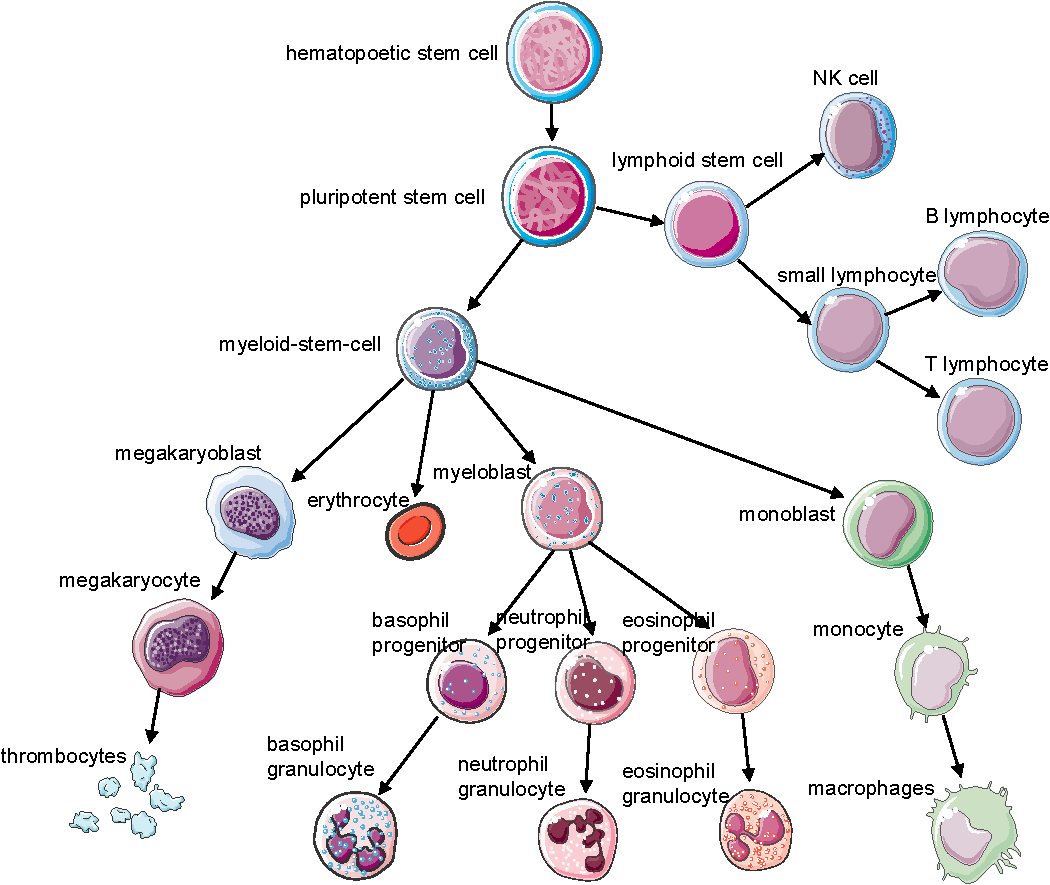
\includegraphics[width=0.95\textwidth]{blood/fig}
	\vspace{0.1cm}
	\caption[hematopoiesis]{hematopoiesis}
	\label{fig:hematopoiesis}
\end{figure}




Thesis Overview
\section{Contributions}
\label{introduction:sec3.contributions}

Contributions

\begin{itemize}
	\item \textbf{A Novel computational method for single cell multi-modal integration:} We derived a computational approach based on canonical correlation analysis(CCA) and correlation test to integrate single cell multi-modal data. The experiment have shown that our method can effectively integrate multiple modalities of single cell to recover the most common signal embedded accoss modalities.

	\item \textbf{A comprehensive evaluation of multi-modal integration methods:} We preceeded a comprehensive evalution for single cell multi-modal integration, invovling: (1) our novel method; (2) seven state-of-the-art integration methods for single cell multi-modalities; In addition, we collected six single cell multi-modal datasets where true labels are available. Moreover, we evaluated the integration results using three metrics as well as the computational resources consuming. Our evaluation represents the most comprehensive comparison for single cell multi-modal integration.

	\item \textbf{A Novel computational method for single cell trajectory inference:} We also derived a computational method based on Delaunay triangulation and graph hodge laplacian decomposition to infer a cell fate tree by performing clustering on paths of single cell data. The experiment have revealed that our approach can accurately detect different branches of single cell data especially for those has complex structured tree single cell data.

	\item \textbf{A series of multiple branches datasets for trajectory inference:} Inspired by PHATE~\citep{moon2017phate}, we constructed 10 datasets with branches number range from 3 to 12 using DLA tree algorthm for the evaluation of different levels of branches single cell data. We further plugged our data into dynverse trajectory inference evaluation system, the datasets covered diverse complexity of single cell data, can be used to further evaluated any new trajectory inference approaches.

	\item \textbf{Evaluation of single cell trajectory inference:} We implmented our method for dynverse evaluation, and also another method STREAM~\citep{chen2019stream} which hasn't been invovled by dynverse. We comprehensively compare our methods with all compared methods.

	\item \textbf{Biological validation with novel single cell Multi-modal data:} We apply our methods MOJITOO and PHLOWRE respectively to integrate and infer trajectories for noval single cell multi-modal kidnay organoid data. Our method can effectively integrate the data and also created cell fate tree.
\end{itemize}


\section{Thesis Structure}
\label{introduction:sec3.structure}
Thesis Structure
